%%%%%%%%%%%%%%%%%%%%%%%%%%%%%%%%%%%%%%%%%%%%%%%%%%%%%%%%%%%%%%%%%%%%%%%%%%%%%%%%%%%%
% Document data
%%%%%%%%%%%%%%%%%%%%%%%%%%%%%%%%%%%%%%%%%%%%%%%%%%%%%%%%%%%%%%%%%%%%%%%%%%%%%%%%%%%%
\documentclass[12pt]{article} %report allows for chapters
%%%%%%%%%%%%%%%%%%%%%%%%%%%%%%%%%%%%%%%%%%%%%%%%%%%%%%%%%%%%%%%%%%%%%%%%%%%%%%%%%%%%
\usepackage{preamble}

\begin{document}

\begin{center}
   \textsc{\large MATH 271, Homework 2, \emph{Solutions}}\\
\end{center}
\vspace{.5cm}

\begin{problem} 
Consider the following autonomous equation.
    \[
    x'=-x^2.
    \]
    \begin{enumerate}[(a)]
        \item Draw the phase line for this system. What are the equilibrium point(s)? Which equilibria are stable? Which are unstable? Explain.
        \item Find a general solution to the ODE.
        \item Explain how your general solution fits the qualitative behavior expected from the phase line. That is, can you show that limits of your general solution match your qualitative analysis?
        \item Can $x(0)=0$ be an initial condition? Explain. \emph{Hint: your analysis from the phase line may prove to be more useful than the general solution you found.}
    \end{enumerate}
\end{problem}
\begin{solution}~
\begin{enumerate}[(a)]
        \item The phase line is as follows:

                \begin{centering}
                \begin{tikzpicture}[thick, scale=3]
                
                    \DrawHorizontalPhaseLine[$x$]{-1,0,1}{}{-0.75, -0.5, -0.25, 0.25,0.5,0.75}
                    \draw [domain=-1:1,smooth,variable=\x,red] plot (\x,-\x*\x);
                \end{tikzpicture}
                \end{centering}
        
        The equilibria are found by setting $x'=0$, hence we have
        \[
            x'=0=x^2
        \]
        and so we have this condition satisfied when $x=0$.  Thus, there is just one equilibrium point.  

        The equilibrium $x=0$ is unstable since $x'$ is negative for $x<0$ and for $x>0$.  In particular, if I choose an initial condition $x(0)>0$, then the particular solution corresponding to this initial condition will limit to $x=0$. If I choose an initial condition $x(0)<0$, then the particular solution corresponding to this initial condition will limit to $-\infty$.  Since solutions do not approach $x=0$ from both sides, $x=0$ can't be stable.  

        \item We have seen this equation arise from studying chemical reactions.  Specifically, this equation could model
\[
2x \xrightarrow{k=1} \to \textrm{Products}.
\]
This equation is also separable.  Which means we can solve by
\begin{align*}
    x'=\frac{dx}{dt}&=-x^2\\
    \iff -\frac{dx}{x^2}&=dt.
\end{align*}
We can then integrate both sides to find
\[
\frac{1}{x}=t+C.
\]
Then we solve for $x$ to find our general solution
\[
\boxed{x=\frac{1}{t+c}.}
\]
\item Let us take the condition $x(0)=1>0$, then our particular solution is then
\[
x(t) = \frac{1}{t+1}.
\]
Now, if we let $t$ increase, then 
\[
\lim_{t \to \infty} x(t) = 0
\]
which agrees with our phase line and analysis from before in part (a).

Likewise, if we take $x(0)=-1<0$, then we have the particular solution
\[
x(t) = \frac{1}{t-1}.
\]
Now, if we let $t$ increase, then we run into an issue when $t=1$ since the denominator goes to zero.  However, we can see that
\[
\lim_{t\to 1^-} x(t) = -\infty.
\]
This again agrees with our phase diagram.

\item Since this equation could model the above reaction, we should expect that the initial condition of $x(0)=0$ works. Why is that? If we start with no reactants (i.e., this initial condition), then no reaction should occur!  We can see that by noting
\[
x'(0)=-x(0)^2=0
\]
which shows that $x'(0)=0$ given this initial condition.  In that case the solution is trivial and no dynamics occur. Said succinctly, starting at an equilibrium point will lead to a steady-state solution where no motion (or in this case, reaction) will occur.

However, just by looking at solving the equation we have from our general solution
\[
x(0)=\frac{1}{0+c}=\frac{1}{c}
\]
it is not really possible to solve this equation. However, if we consider something like the $\lim_{c\to \infty} \frac{1}{t+c}=0$ then this may make some sense.  Below is a graph of many different values of $c$. Notice that they approach the case $x(t)=0$ as a solution as $t\to \infty$. So in the case that $x(0)=0$ the particular solution would be
\[
\boxed{x(t)=0.}
\]
\begin{figure}[H]
    \centering
    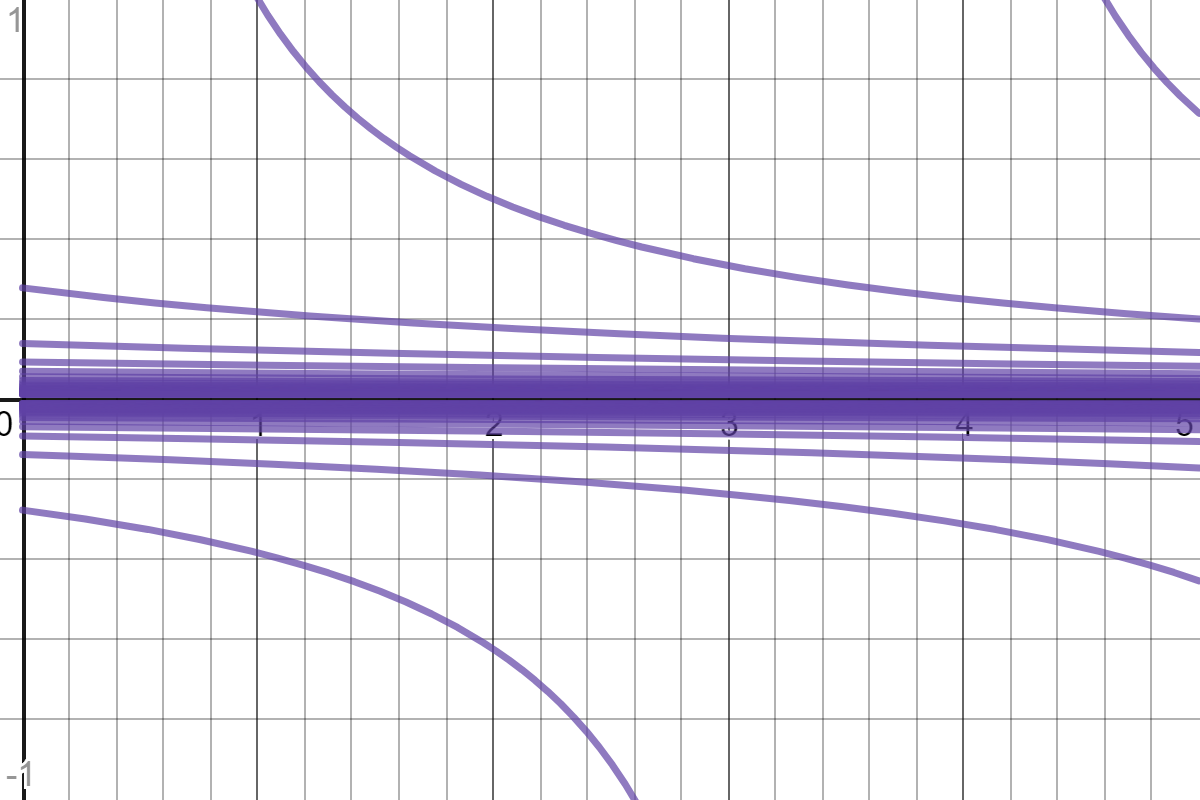
\includegraphics[width=\textwidth]{2nd_order_chem.png}
\end{figure}
\end{enumerate}
\end{solution}



\newpage
\begin{problem}
Let $y$ be a function of $x$ and consider the following differential equation.
\[
y' = y\cos(x).
\]
\begin{enumerate}[(a)]
    \item What is the order of this equation? Is the equation separable? Explain.
    \item Plot an approximation of the slope field for this equation using this Desmos link: \url{https://www.desmos.com/calculator/e93gktwtfo}. \emph{Note that you will have to modify the $g(x,y)$ equation in that page.}
    \item Find the general solution to this equation.
    \item Given the initial data $y(0)=1$, find the particular solution.
    \item Plot this function over your slope field. Explain how you could have approximated this solution using just the slope field.
    \item Explain in words what the solution describes if we let $y(x)$ be the position of some object and $x$ represents time.
\end{enumerate}
\end{problem}
\begin{solution}~
\begin{enumerate}[(a)]
    \item This is a first order equation that is also separable. To see that it is separable since we need to have 
    \[
        y' = f(x)g(y).
    \]
    Here, we can let $f(x)=\cos(x)$ and $g(y)=y$ to write our equation in a separable form.
    \item Here is an approximation of the slope field for this equation:
    \begin{figure}[H]
        \centering
        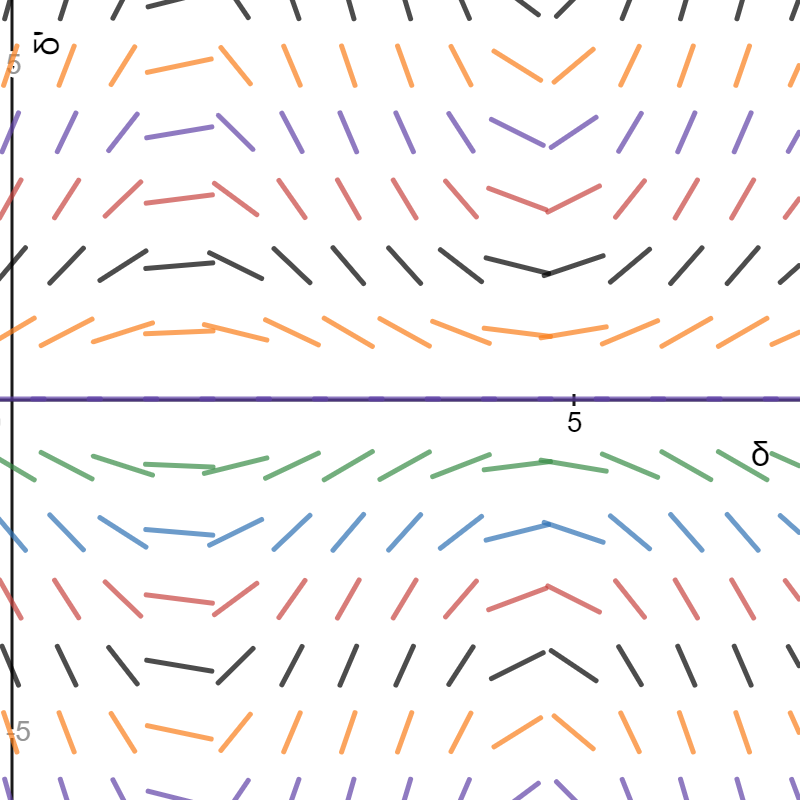
\includegraphics[width=.5\textwidth]{slope_field.png}
        \caption{Slope field for the equation $y'=y\cos(x)$.}
    \end{figure}
    \item We can find the general solution by 
    \begin{align*}
        \frac{dy}{dx}&= y\cos(x)\\
        \int \frac{1}{y}dy &= \int \cos(x)dx\\
        \ln(y)&=\sin(x)+C.
    \end{align*}
    Then we solve for $y$ to find
    \begin{align*}
        y&=e^{\sin(x)+C}=e^C \cdot e^{\sin(x)}\\
        &= Ae^{\sin(x)},
    \end{align*}
    which is our general solution.
    \item If we have $y(0)=1$ then we plug this into our general solution
    \[
    1=x(0)=Ae^{\sin(0)}=A
    \]
    so that $A=1$. Thus the particular solution is
    \[
    \boxed{y(x)=Ae^{\sin(x)}.}
    \]

    We can plot this solution over the slope field as follows:
    \begin{figure}[H]
        \centering
        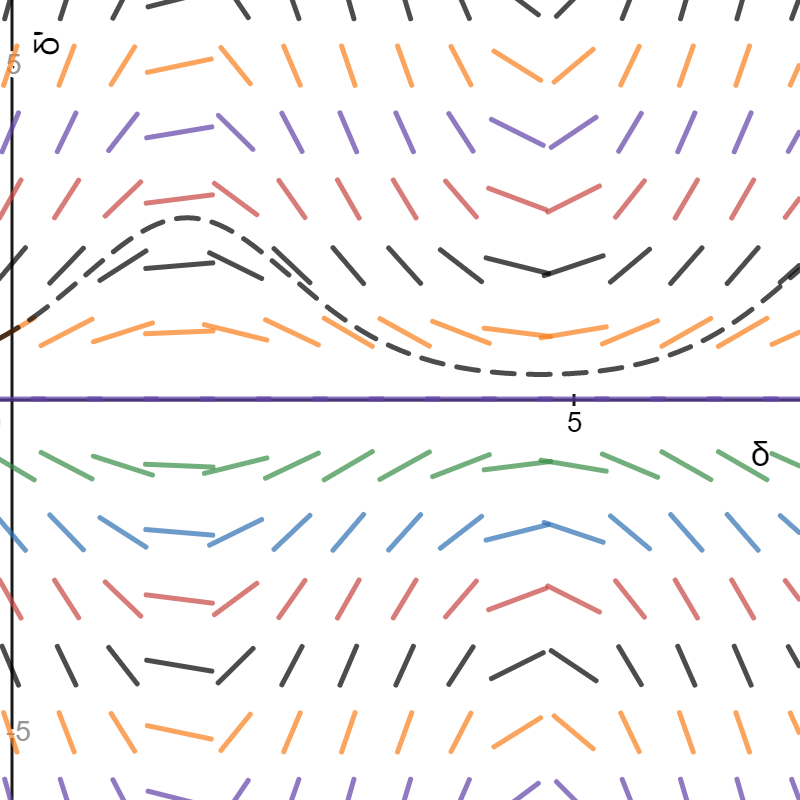
\includegraphics[width=.5\textwidth]{slope_field_solution.png}  
        \caption{The particular solution $y(x)=e^{\sin(x)}$ (in dashed black) plotted over the previous slope field.}
    \end{figure}
    \item The solution represents a system that oscillates back and forth. However, it is not oscillation as we see with a Hookean spring and a mass system.  In this case, this would a oscillation due to something else entirely. Notice, for example, that the valleys and peaks are not the same width.
\end{enumerate}
\end{solution}

\newpage
\begin{problem}
Consider the differential equation
\[
x'=\frac{x+t}{t}.
\]
\begin{enumerate}[(a)]
    \item Let $f(x,t)=\frac{x+t}{t}$. Show that $f(x,t)=f(\lambda x, \lambda t)$.
    \item Given (a) holds, use the change of variables $u=\frac{x}{t}$ to rewrite the differential equation as a separable equation in terms of $u$.
    \item Find the general solution to the equation and write your solution in terms of the original variables $t$ and $x$.
\end{enumerate}
\end{problem}
\begin{solution}~
\begin{enumerate}[(a)]
    \item To show this, we check to see if the equality is true by 
    \begin{align*}
        f(\lambda x, \lambda t) &= \frac{\lambda x + \lambda t}{\lambda t}\\
        &= \frac{\lambda(x+t)}{\lambda t}\\
        &= \frac{x+t}{t}\\
        &= f(t).
    \end{align*}
    So the property holds, which leads us to (b).
    \item Now, we let $u=\frac{x}{t}$ which allows us to say $x=tu$.  We can then take
    \[
    x' = f(x,t) = f(tu,t)=\frac{tu+t}{t}=\frac{t(u+1)}{t}=u+1.
    \]
    Given our substitution, we can also take
    \[
    x'=(tu)'=u+tu'
    \]
    and substitute this back in our other expression to get
    \[
    u+tu'=u+1.
    \]
    We can simplify this a bit
    \begin{align*}
        u+tu'&=u+1\\
        tu'&= 1\\
        u'&=\frac{1}{t}.
    \end{align*}
    This is a separable equation.
    \item Now we can solve the previous equation using separation. So we have
    \begin{align*}
        \frac{du}{dt}&= \frac{1}{t}\\
        \int du &= \int \frac{dt}{t}\\
        u&= \ln(t)+C.
    \end{align*}
    Recall that we let $u=\frac{x}{t}$ and to get back to the original variable we need to solve for $x$. So we take
    \begin{align*}
        u=\frac{x}{t}&=\ln(t)+C\\
        x&=t\ln(t)+Ct.
    \end{align*}
    So the general solution to our original equation is
    \[
    \boxed{x(t)=t\ln(t)+Ct.}
    \]
\end{enumerate}
\end{solution}

\newpage
\begin{problem}
Find the general solution to the following equation.
\[
tx'+2x=\frac{\sin(t)}{t}.
\]
Show that your solution is correct. (\emph{Hint: can you use an integrating factor?})
\end{problem}
\begin{solution}
Note that this is a first order linear equation if we divide the whole expression by $t$. We can see this by,
\begin{align*}
    tx'+2x&=\frac{\sin(t)}{t}\\
    x'+\frac{2}{t}x&=\frac{\sin(t)}{t^2}.
\end{align*}
This matches the form of a first order linear equation which is typically written as
\[
x'+f(t)x=g(t).
\]
So note that in our case, $f(t)=\frac{2}{t}$ and $g(t)=\frac{\sin(t)}{t^2}$. Given that, we can solve this equation using the integrating factor technique.  For that, we have the integrating factor
\begin{align*}
\mu &= e^{\int f(t)dt}\\
&=e^{\int \frac{2}{t}dt}\\
&= e^{2\ln(t)}\\
&=e^{\ln\left(t^2\right)}\\
&=t^2.
\end{align*}
Now, we have $\mu$ and we can find $x(t)$ by
\begin{align*}
    x&= \frac{1}{\mu(t)}\int \mu(t)g(t)dt\\
    &= \frac{1}{t^2} \int t^2 \frac{\sin(t)}{t^2}dt\\
    &= \frac{1}{t^2}\int \sin(t)dt\\
    &= -\frac{1}{t^2} \cos(t)+\frac{C}{t^2}.
\end{align*}
So our general solution is
\[
\boxed{x(t)=-\frac{1}{t^2}\cos(t)+\frac{C}{t^2}.}
\]
\end{solution}

\end{document}